\documentclass[12pt,a4paper]{article}
\usepackage[utf8]{inputenc}
\usepackage[english]{babel}
\usepackage{geometry}
\usepackage{fancyhdr}
\usepackage{graphicx}
\usepackage{longtable}
\usepackage{array}
\usepackage{booktabs}
\usepackage{xcolor}
\usepackage{hyperref}
\usepackage{listings}
\usepackage{enumitem}
\usepackage{float}
\usepackage{microtype}

% Fix headheight
\setlength{\headheight}{14.5pt}

% Add microtype for better text fitting
\usepackage{microtype}

% Add proper quotes
\newcommand{\qq}[1]{``#1''}

% Add missing author
\title{%
    \vspace{-1cm}
    \textbf{Final Release Document\\HIV Clinic Management System}
}
\author{Development Team}
\date{January 2025 --- Ho Chi Minh City}

% Adjust margins for better text fit
\geometry{margin=1in,top=1.2in}

\pagestyle{fancy}
\fancyhf{}
\rhead{\thepage}
\lhead{HIV Clinic Final Release}

\begin{document}

\maketitle
\thispagestyle{empty}

\newpage

\section*{Record of Changes}

\begin{longtable}{@{}|p{2cm}|p{2cm}|p{1cm}|p{3cm}|p{6cm}|@{}}
\hline
\textbf{Version} & \textbf{Date} & \textbf{A*M, D} & \textbf{In charge} & \textbf{Change Description} \\
\hline
V1.0 & 07/01/2025 & A & Development Team & Initial Final Release document for HIV Clinic Management System \\
\hline
\end{longtable}

\textit{*A - Added M - Modified D - Deleted}

\newpage

\tableofcontents

\newpage

\section{Deliverable Package}

This section lists all source programs, scripts, and documents included in the HIV Clinic Management System release.

\begin{longtable}{@{}|p{1cm}|p{6cm}|p{7cm}|@{}}
\hline
\textbf{No.} & \textbf{File} & \textbf{Notes} \\
\hline
1 & schema.sql & Database schema including table structures for all entities \\
\hline
2 & data.sql & Initial data including user accounts, roles, and sample data \\
\hline
3 & RDS\_Document\_HIV\_Clinic\_Filled.tex & Final Requirements and Design Specification Document \\
\hline
4 & SDS\_HIV\_Clinic\_LaTeX.tex & Final Software Design Specification Document \\
\hline
5 & Project\_Tracking\_HIV\_Clinic\_LaTeX.tex & Complete project tracking with sprint iterations \\
\hline
6 & Issues\_Report\_HIV\_Clinic\_LaTeX.tex & Final issues tracking report for the entire project \\
\hline
7 & pom.xml & Maven project configuration with dependencies \\
\hline
8 & package.json & Frontend dependencies and build configuration \\
\hline
9 & HivClinicBackendApplication.java & Spring Boot main application class \\
\hline
10 & Source Code (Backend) & Complete Spring Boot backend with REST API \\
\hline
11 & Source Code (Frontend) & Complete React frontend application \\
\hline
12 & setup-database.bat & Database setup script for Windows \\
\hline
13 & start-application.sh & Application startup script for Linux/Mac \\
\hline
14 & README.md & Project documentation and setup instructions \\
\hline
\end{longtable}

\subsection{Project Information}

\begin{itemize}
    \item \textbf{Project Name:} HIV Clinic Management System
    \item \textbf{Version:} 1.0.0
    \item \textbf{Release Date:} January 2025
    \item \textbf{Technology Stack:} Spring Boot 3.2.0, React 18.2.0, Microsoft SQL Server
    \item \textbf{Repository:} https://github.com/ruskicoder/swp-hiv-clinic
\end{itemize}

\subsection{Other Related Deliverables}

\begin{itemize}
    \item \textbf{Source Code Repository:} https://github.com/ruskicoder/swp-hiv-clinic
    \item \textbf{Frontend Application:} http://localhost:3000
    \item \textbf{Backend API:} http://localhost:8080/api
    \item \textbf{Database:} Microsoft SQL Server (hiv\_clinic database)
\end{itemize}

\section{Installation Guides}

This section provides comprehensive installation instructions for setting up the HIV Clinic Management System.

\subsection{System Requirements}

\begin{longtable}{@{}|p{3cm}|p{3cm}|p{8cm}|@{}}
\hline
\textbf{Component} & \textbf{Version} & \textbf{Description} \\
\hline
Java JDK & 17+ & Required for Spring Boot backend \\
\hline
Node.js & 18+ & Required for React frontend \\
\hline
Maven & 3.9+ & Build tool for Java backend \\
\hline
SQL Server & 2019+ & Database server (Express edition acceptable) \\
\hline
Git & Latest & Version control system \\
\hline
\end{longtable}

\subsection{Backend Installation}

\begin{enumerate}
    \item \textbf{Clone the Repository:}
    \begin{lstlisting}[language=bash]
git clone https://github.com/ruskicoder/swp-hiv-clinic.git
cd swp-hiv-clinic
    \end{lstlisting}
    
    \item \textbf{Configure Database:}
    \begin{itemize}
        \item Install Microsoft SQL Server
        \item Create database named \texttt{hiv\_clinic}
        \item Update connection string in \texttt{src/main/resources/application.properties}
    \end{itemize}
    
    \item \textbf{Run Database Setup:}
    \begin{lstlisting}[language=bash]
# For Windows
setup-database.bat

# For Linux/Mac
chmod +x setup-database.sh
./setup-database.sh
    \end{lstlisting}
    
    \item \textbf{Build and Run Backend:}
    \begin{lstlisting}[language=bash]
mvn clean install
mvn spring-boot:run
    \end{lstlisting}
    
    \item \textbf{Verify Backend Installation:}
    \begin{itemize}
        \item Backend starts on port 8080
        \item Health check: \texttt{http://localhost:8080/api/health}
        \item API documentation: \texttt{http://localhost:8080/api}
    \end{itemize}
\end{enumerate}

\subsection{Frontend Installation}

\begin{enumerate}
    \item \textbf{Install Dependencies:}
    \begin{lstlisting}[language=bash]
npm install
    \end{lstlisting}
    
    \item \textbf{Configure Environment:}
    \begin{itemize}
        \item Create \texttt{.env} file if needed
        \item Verify API endpoint configuration
    \end{itemize}
    
    \item \textbf{Start Frontend:}
    \begin{lstlisting}[language=bash]
npm run dev
    \end{lstlisting}
    
    \item \textbf{Verify Frontend Installation:}
    \begin{itemize}
        \item Frontend starts on port 3000
        \item Application available at: \texttt{http://localhost:3000}
    \end{itemize}
\end{enumerate}

\subsection{Database Setup}

\begin{enumerate}
    \item \textbf{Create Database:}
    \begin{lstlisting}[language=sql]
CREATE DATABASE hiv_clinic;
USE hiv_clinic;
    \end{lstlisting}
    
    \item \textbf{Execute Schema:}
    \begin{itemize}
        \item Run \texttt{src/main/resources/db/schema.sql}
        \item This creates all required tables and relationships
    \end{itemize}
    
    \item \textbf{Load Initial Data:}
    \begin{itemize}
        \item Run \texttt{src/main/resources/db/data.sql}
        \item This creates default user accounts and sample data
    \end{itemize}
\end{enumerate}

\subsection{Quick Start Script}

For easy deployment, use the provided startup script:

\begin{lstlisting}[language=bash]
# Make script executable
chmod +x start-application.sh

# Start both backend and frontend
./start-application.sh

# Start only backend
./start-application.sh backend

# Start only frontend  
./start-application.sh frontend

# Stop all services
./start-application.sh stop
\end{lstlisting}

\section{User Manual}

This section provides comprehensive user guidance for the HIV Clinic Management System.

\subsection{Overview}

The HIV Clinic Management System is a comprehensive web application designed to manage HIV patient care, appointments, and treatment workflows. The system supports four main user roles with specific access levels and functionalities.

\subsubsection{System Architecture}

\begin{itemize}
    \item \textbf{Frontend:} React 18.2.0 single-page application
    \item \textbf{Backend:} Spring Boot 3.2.0 REST API
    \item \textbf{Database:} Microsoft SQL Server with normalized schema
    \item \textbf{Authentication:} JWT token-based security
    \item \textbf{Authorization:} Role-based access control (RBAC)
\end{itemize}

\subsubsection{User Roles}

\begin{longtable}{@{}|p{2cm}|p{4cm}|p{8cm}|@{}}
\hline
\textbf{Role} & \textbf{Primary Functions} & \textbf{Key Responsibilities} \\
\hline
Patient & Personal health management & View appointments, manage profile, receive medication reminders \\
\hline
Doctor & Patient care delivery & Manage appointments, update patient records, prescribe treatments \\
\hline
Admin & System administration & Manage users, system settings, full access to all features \\
\hline
Manager & Clinic operations & Oversee operations, generate reports, manage staff \\
\hline
\end{longtable}

\subsection{Authentication and Access}

\subsubsection{Login Process}

\begin{enumerate}
    \item Navigate to \texttt{http://localhost:3000}
    \item Enter your username and password
    \item Click "Login" button
    \item System redirects to role-appropriate dashboard
\end{enumerate}

\subsubsection{Default User Accounts}

\begin{longtable}{@{}|p{2cm}|p{3cm}|p{3cm}|p{6cm}|@{}}
\hline
\textbf{Role} & \textbf{Username} & \textbf{Password} & \textbf{Description} \\
\hline
Admin & admin & admin123 & System administrator with full access \\
\hline
Doctor & doctor1 & doctor123 & Test doctor account for demonstration \\
\hline
Patient & patient1 & patient123 & Test patient account for demonstration \\
\hline
Manager & manager1 & manager123 & Test manager account for demonstration \\
\hline
\end{longtable}

\subsection{Patient Workflow}

\subsubsection{Patient Registration}

\begin{enumerate}
    \item Click "Register" on login page
    \item Fill in personal information:
    \begin{itemize}
        \item Username (unique)
        \item Email address
        \item Password (minimum 8 characters)
        \item First and Last name
        \item Contact information
    \end{itemize}
    \item Select "Patient" role
    \item Submit registration form
    \item Account activation (if required)
\end{enumerate}

\subsubsection{Appointment Booking}

\begin{enumerate}
    \item Login to patient dashboard
    \item Click "Book Appointment"
    \item Select preferred doctor from dropdown
    \item Choose appointment date using calendar
    \item Select available time slot
    \item Add appointment notes (optional)
    \item Confirm booking
    \item Receive appointment confirmation
\end{enumerate}

\begin{figure}[H]
\centering
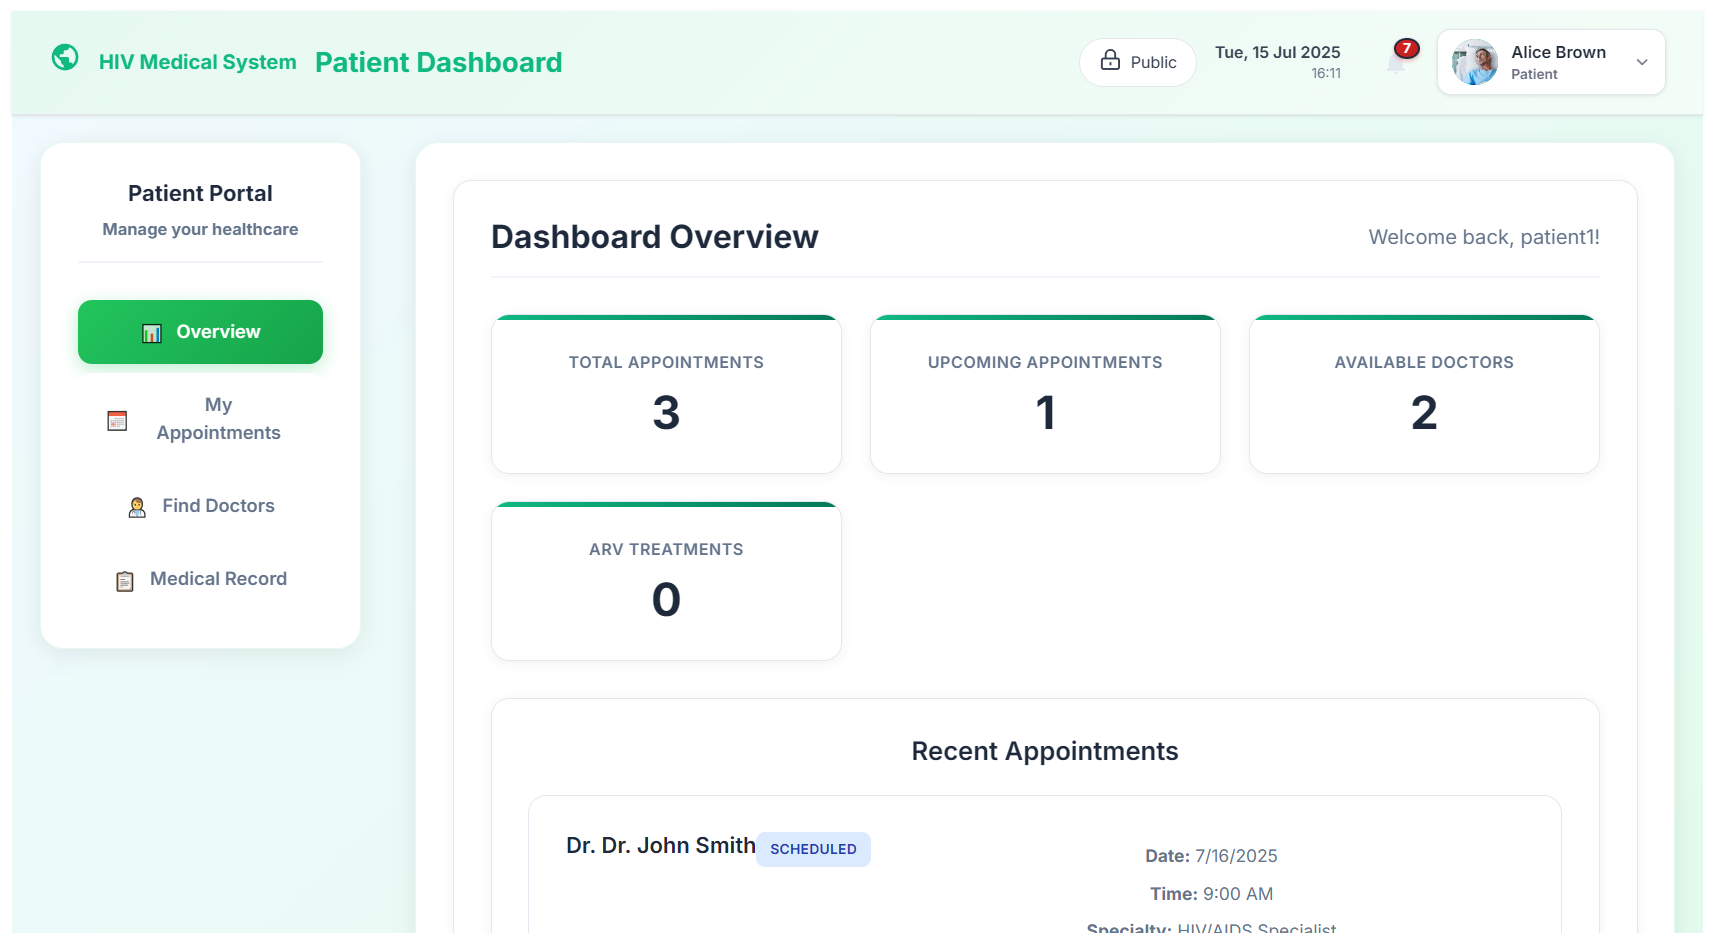
\includegraphics[width=0.9\textwidth]{images/patient_login.png}
\caption{Patient Login Interface}
\label{fig:patient-login}
\end{figure}

\begin{figure}[H]
\centering
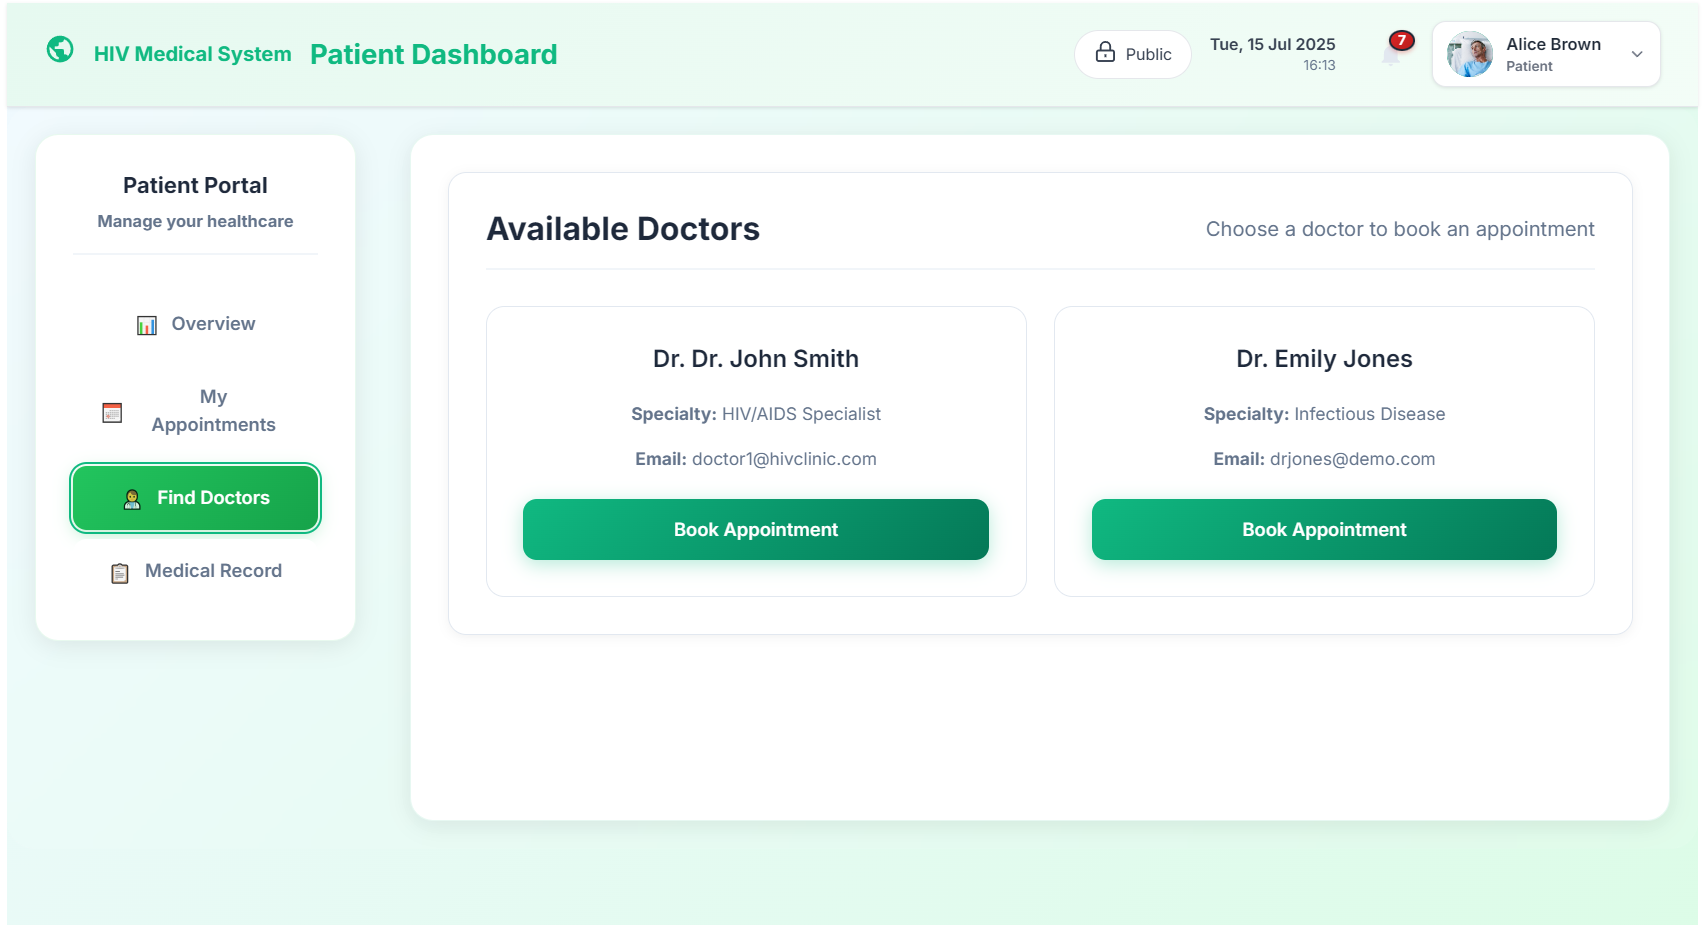
\includegraphics[width=0.9\textwidth]{images/patient_register.png}
\caption{Patient Registration Interface}
\label{fig:patient-register}
\end{figure}

\begin{figure}[H]
\centering
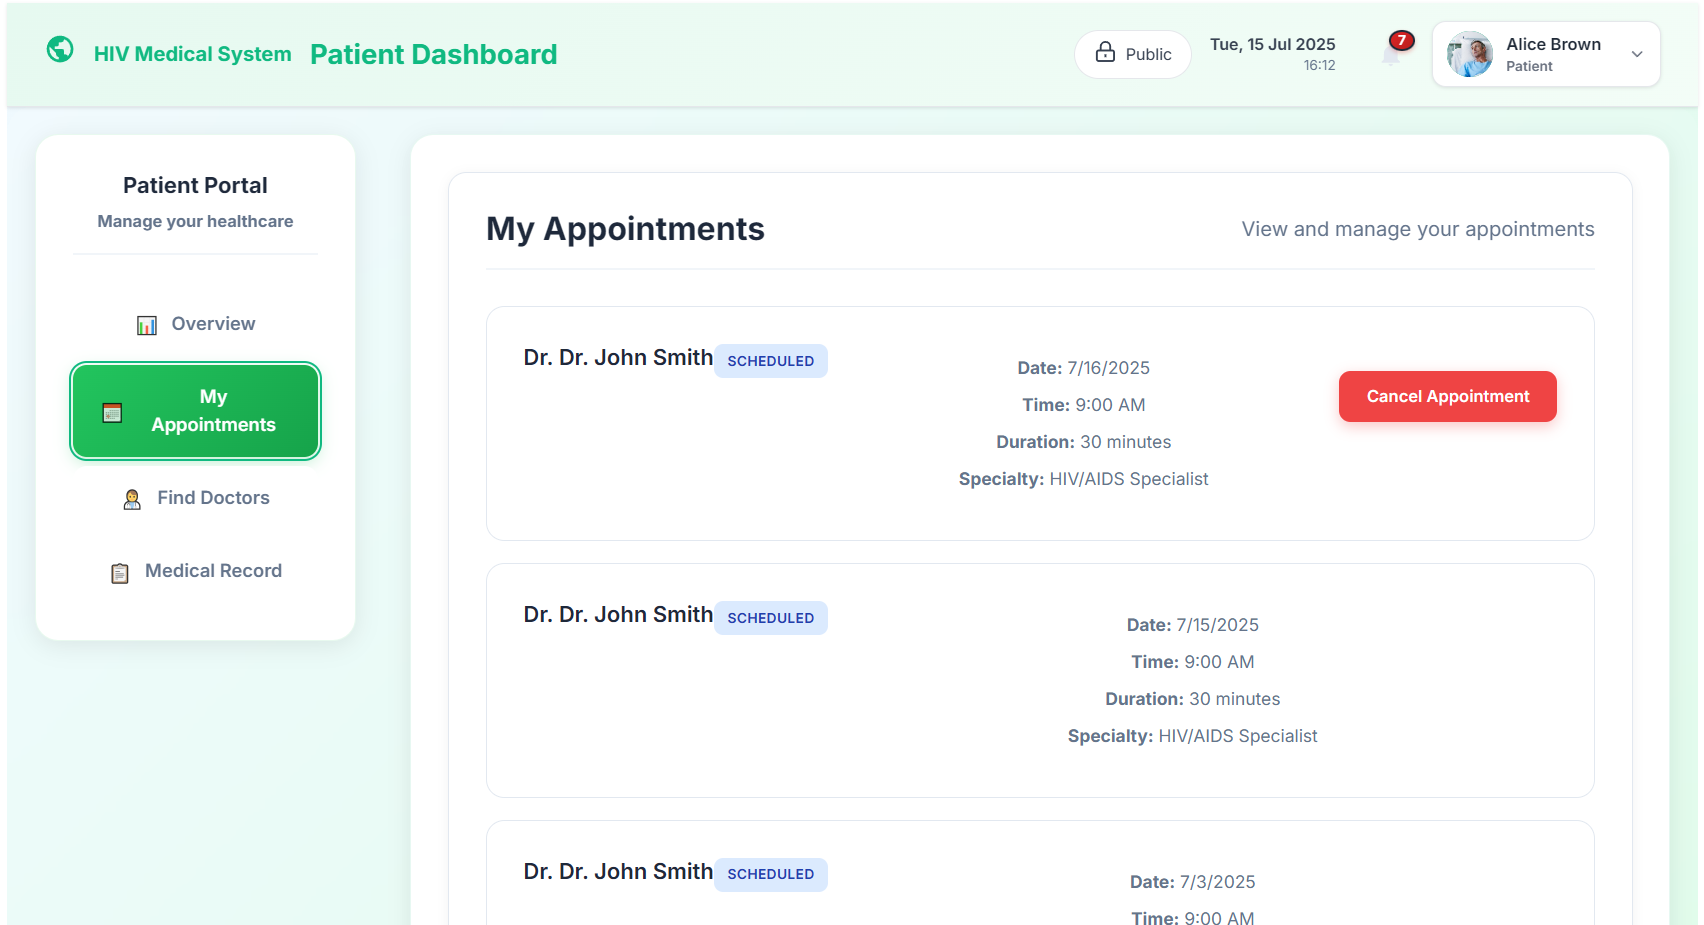
\includegraphics[width=0.9\textwidth]{images/patient_booking.png}
\caption{Patient Appointment Booking Interface}
\label{fig:patient-booking}
\end{figure}

\begin{figure}[H]
\centering
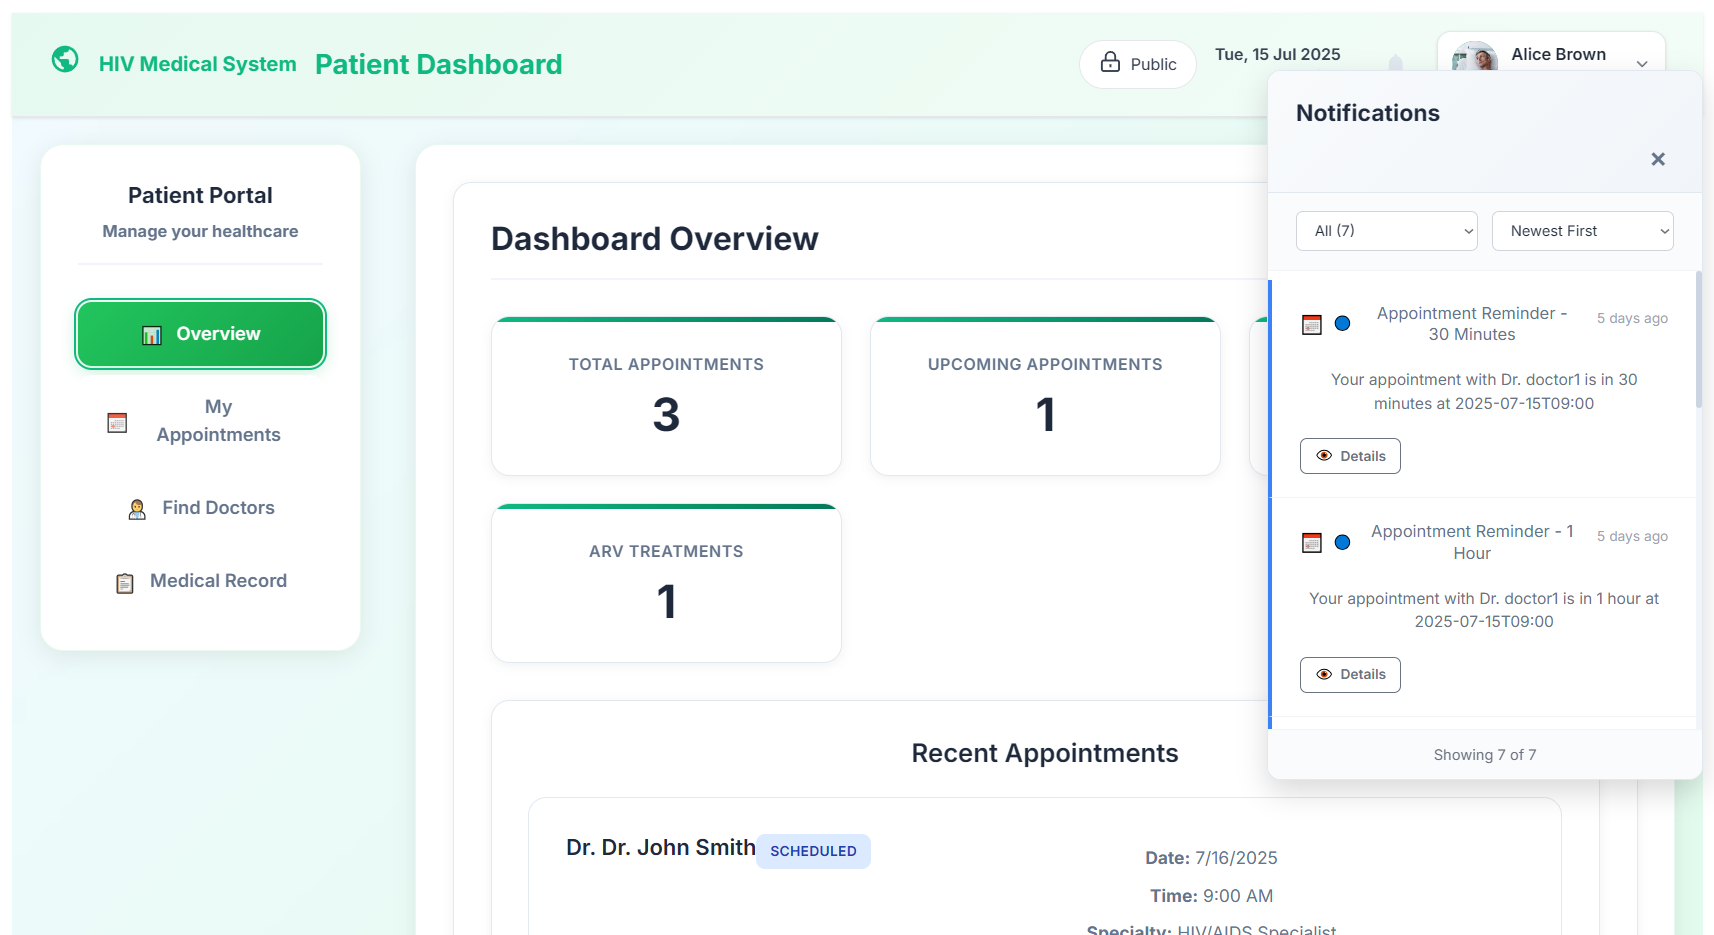
\includegraphics[width=0.9\textwidth]{images/patient_dashboard.png}
\caption{Patient Dashboard Interface}
\label{fig:patient-dashboard}
\end{figure}

\begin{figure}[H]
\centering
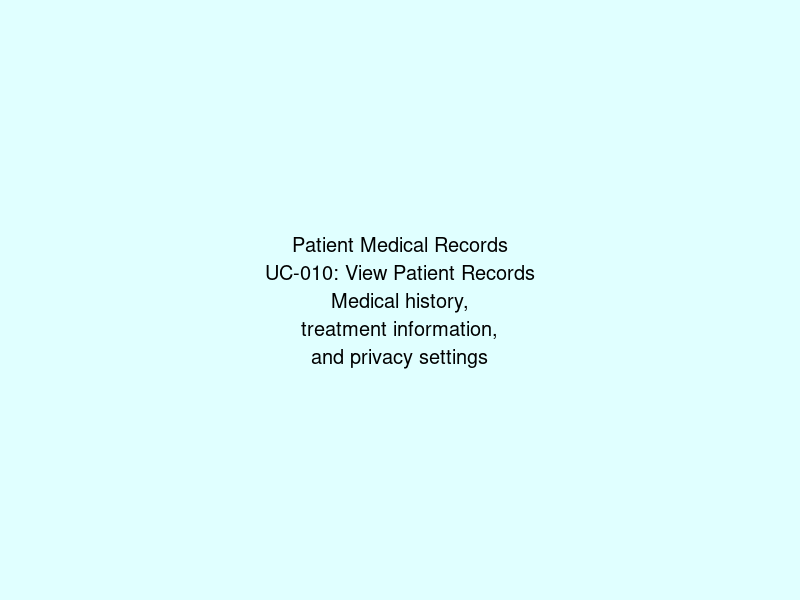
\includegraphics[width=0.9\textwidth]{images/patient_records.png}
\caption{Patient Medical Records Interface}
\label{fig:patient-records}
\end{figure}

\subsection{Doctor Workflow}

\subsubsection{Availability Management}

\begin{enumerate}
    \item Login to doctor dashboard
    \item Click "Manage Availability"
    \item Select dates for availability
    \item Set time slots (start and end times)
    \item Save availability schedule
    \item View and edit existing slots
\end{enumerate}

\begin{figure}[H]
\centering
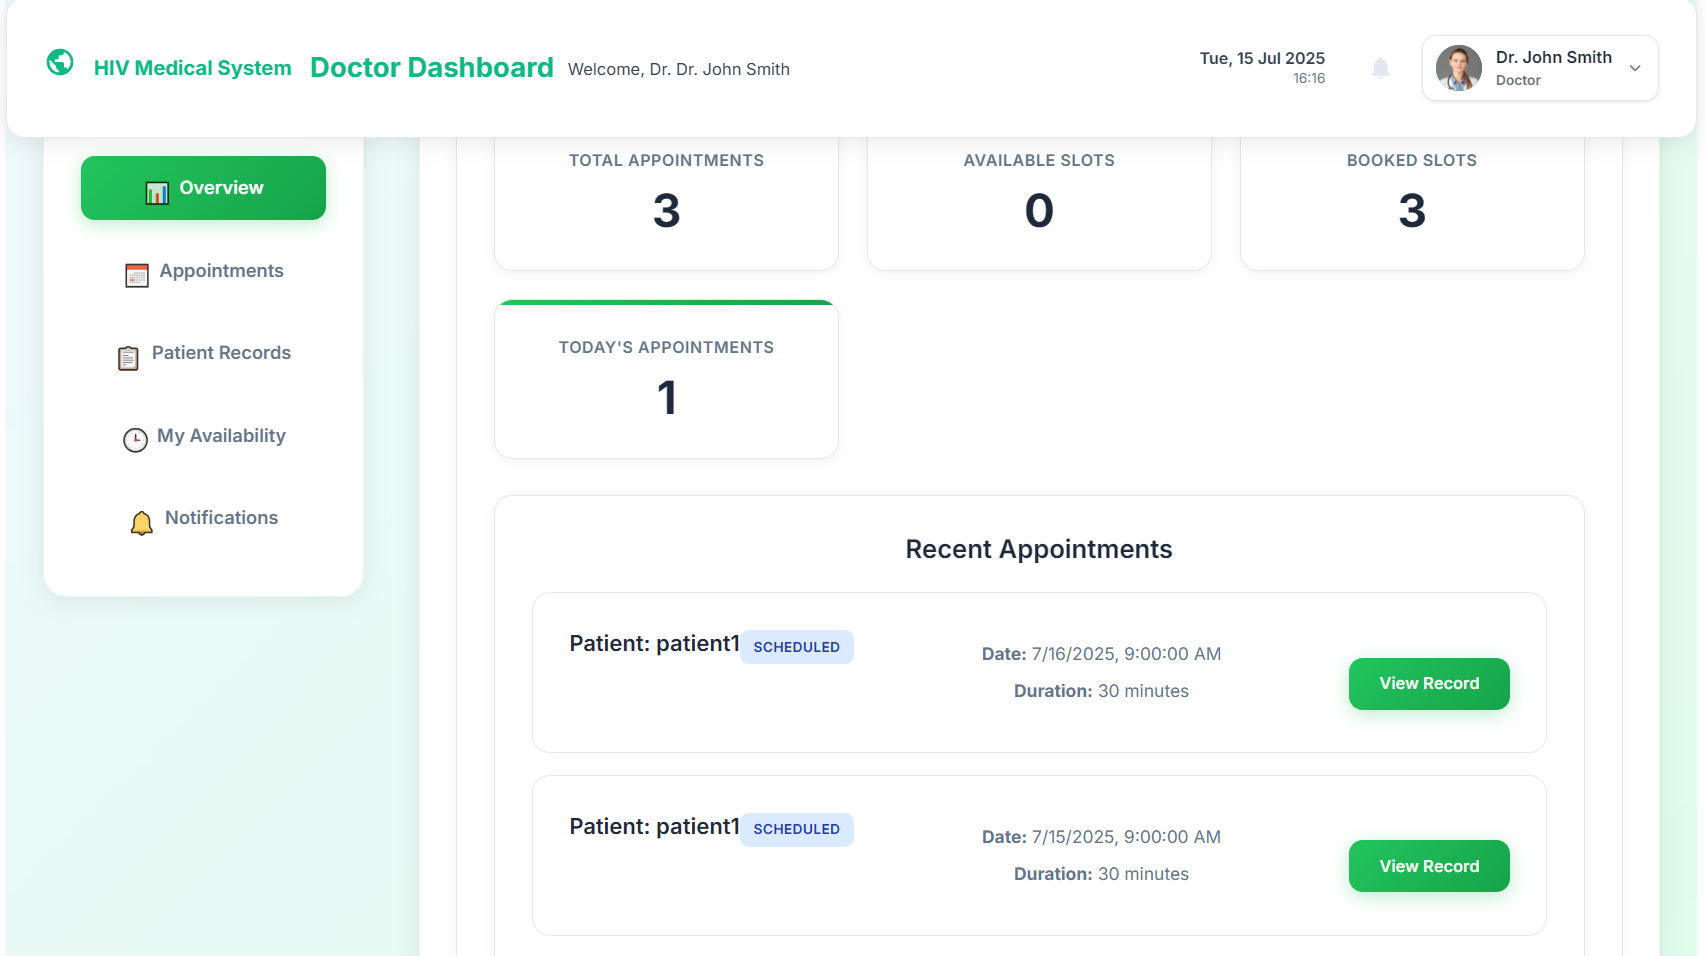
\includegraphics[width=0.9\textwidth]{images/doctor_login.png}
\caption{Doctor Login Interface}
\label{fig:doctor-login}
\end{figure}

\begin{figure}[H]
\centering
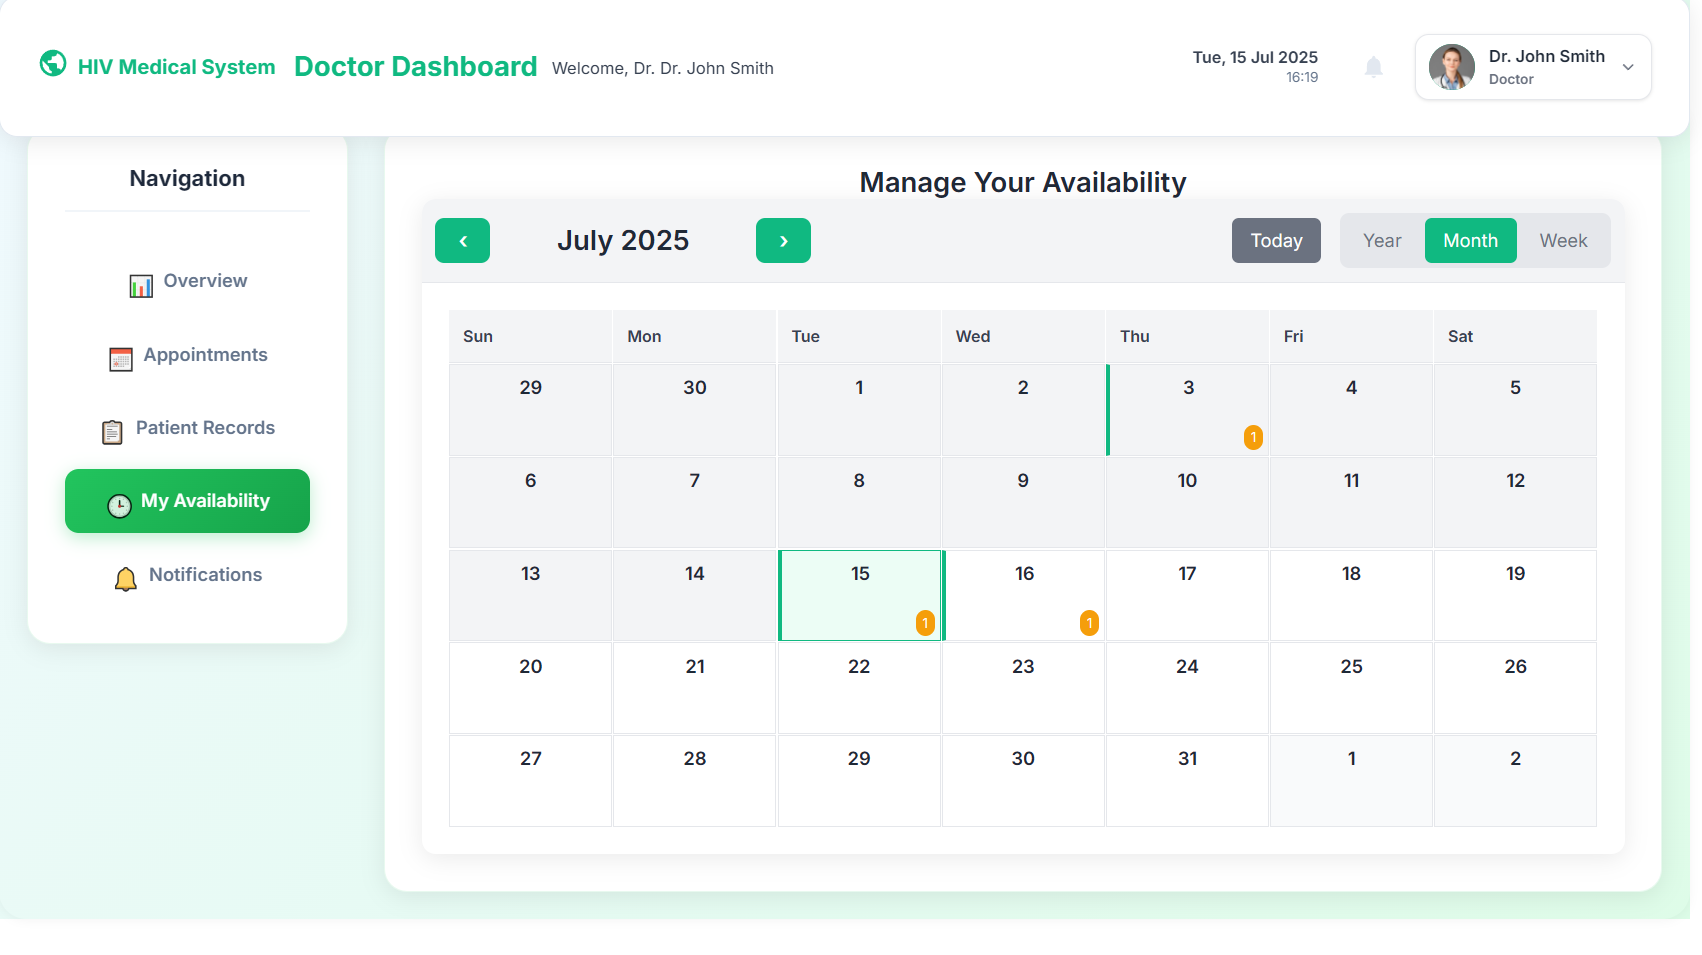
\includegraphics[width=0.9\textwidth]{images/doctor_availability.png}
\caption{Doctor Availability Management Interface}
\label{fig:doctor-availability}
\end{figure}

\begin{figure}[H]
\centering
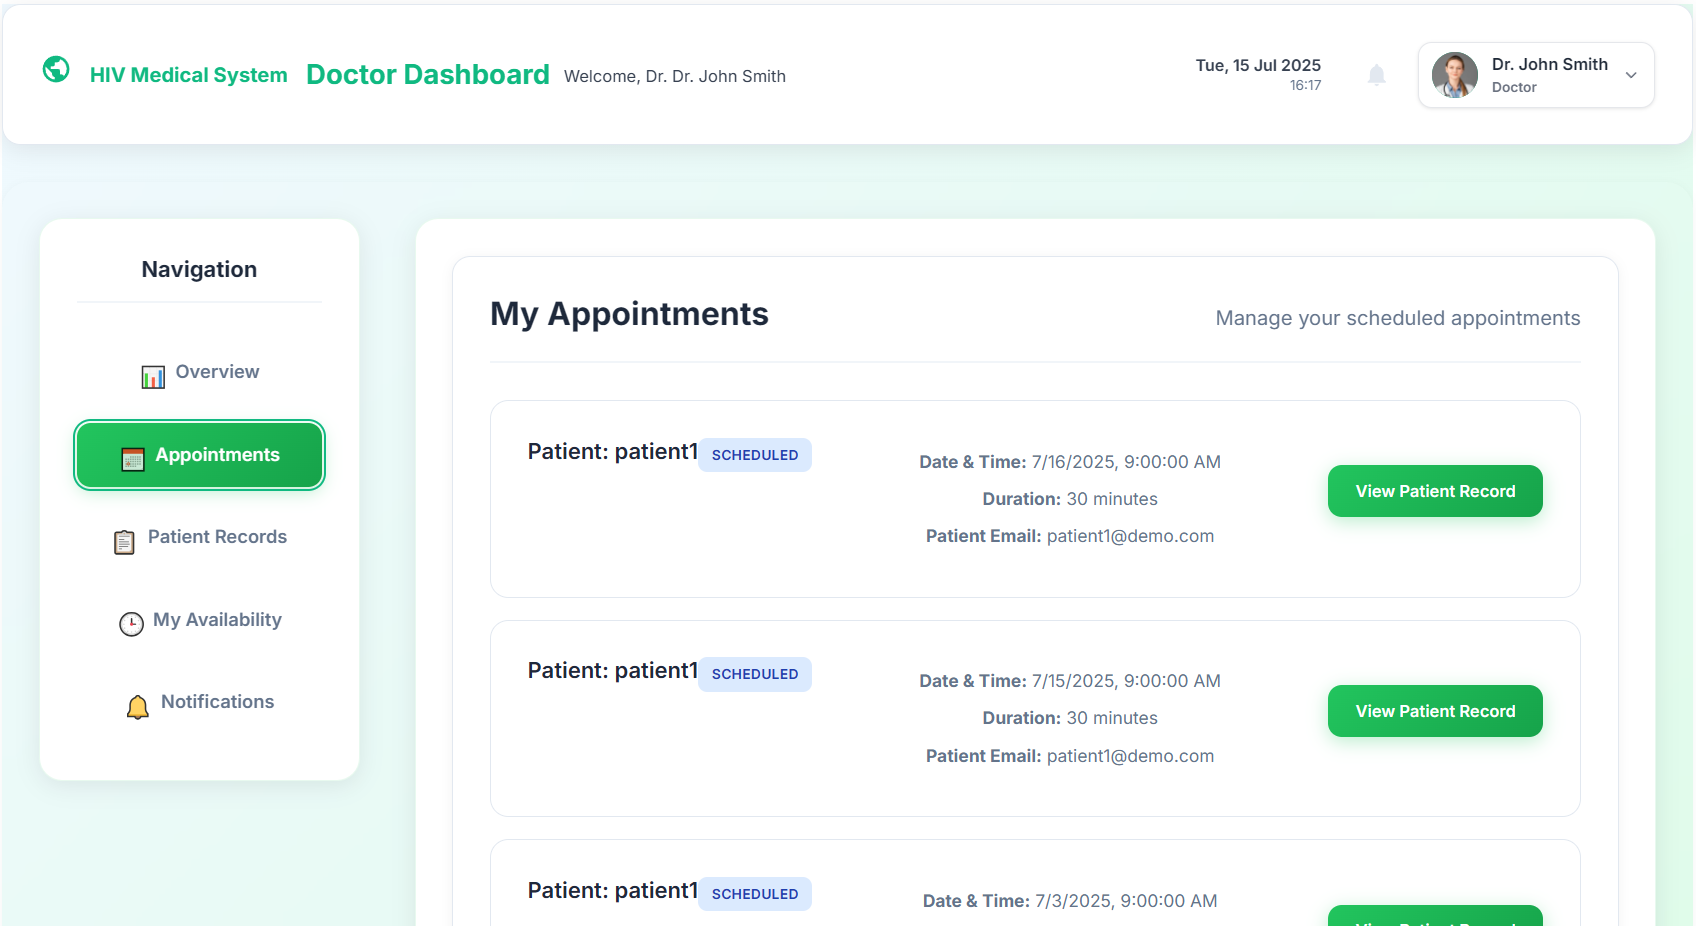
\includegraphics[width=0.9\textwidth]{images/doctor_dashboard.png}
\caption{Doctor Dashboard Interface}
\label{fig:doctor-dashboard}
\end{figure}

\begin{figure}[H]
\centering
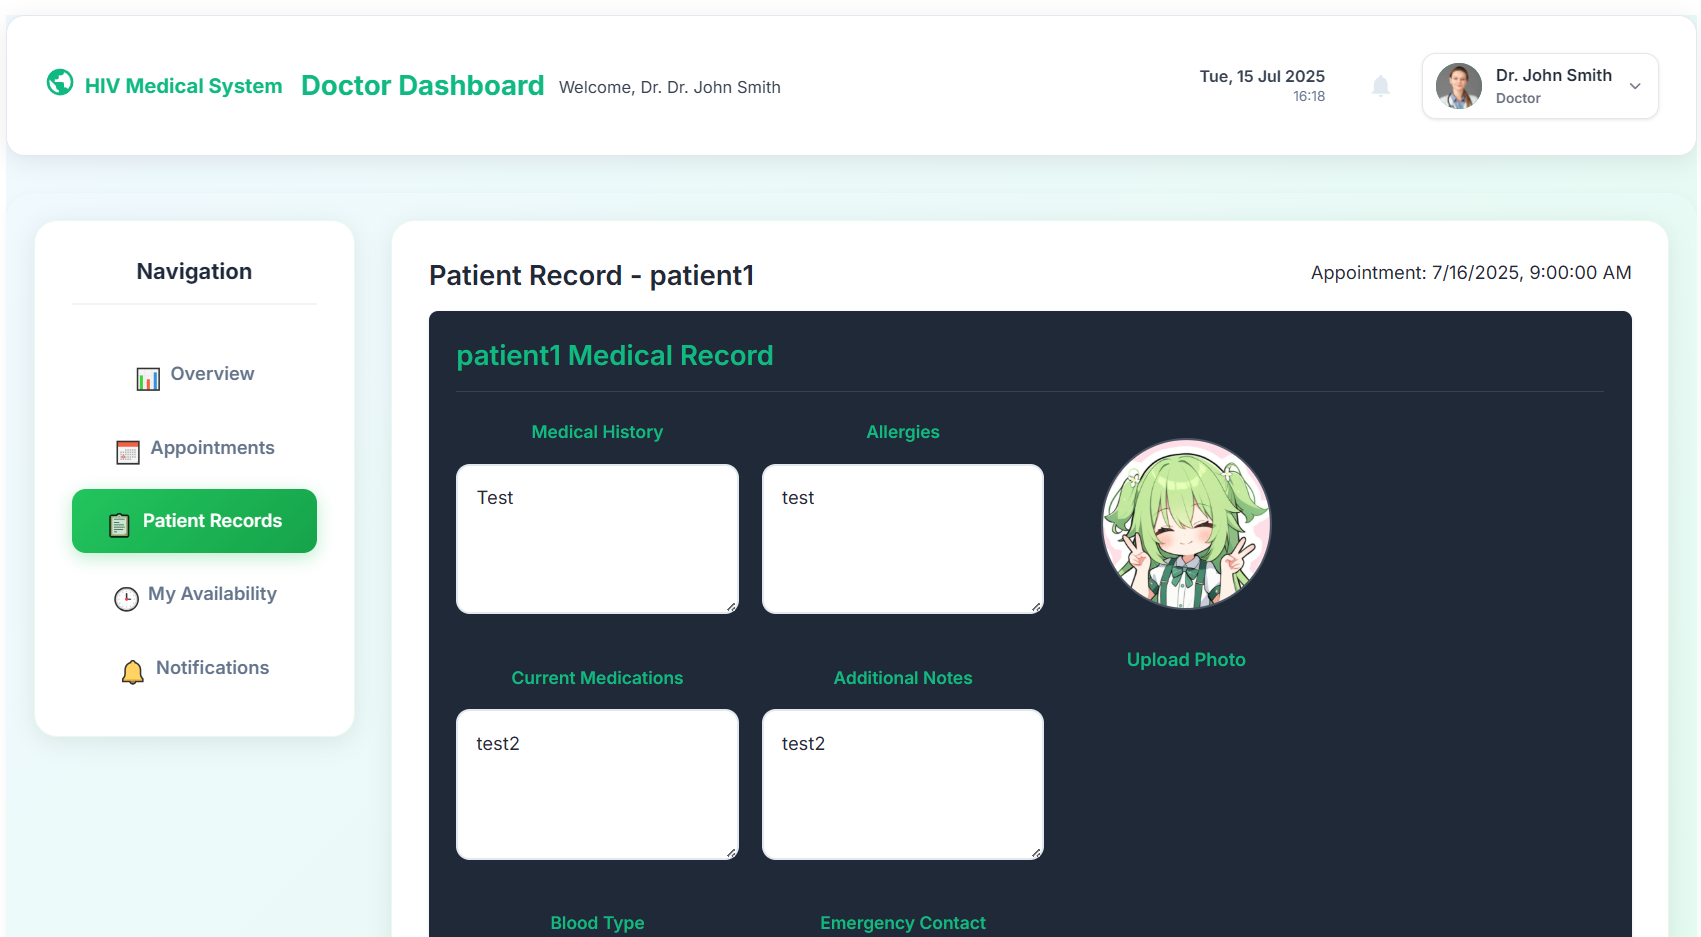
\includegraphics[width=0.9\textwidth]{images/doctor_patientview.png}
\caption{Doctor Patient View Interface}
\label{fig:doctor-patientview}
\end{figure}

\begin{figure}[H]
\centering
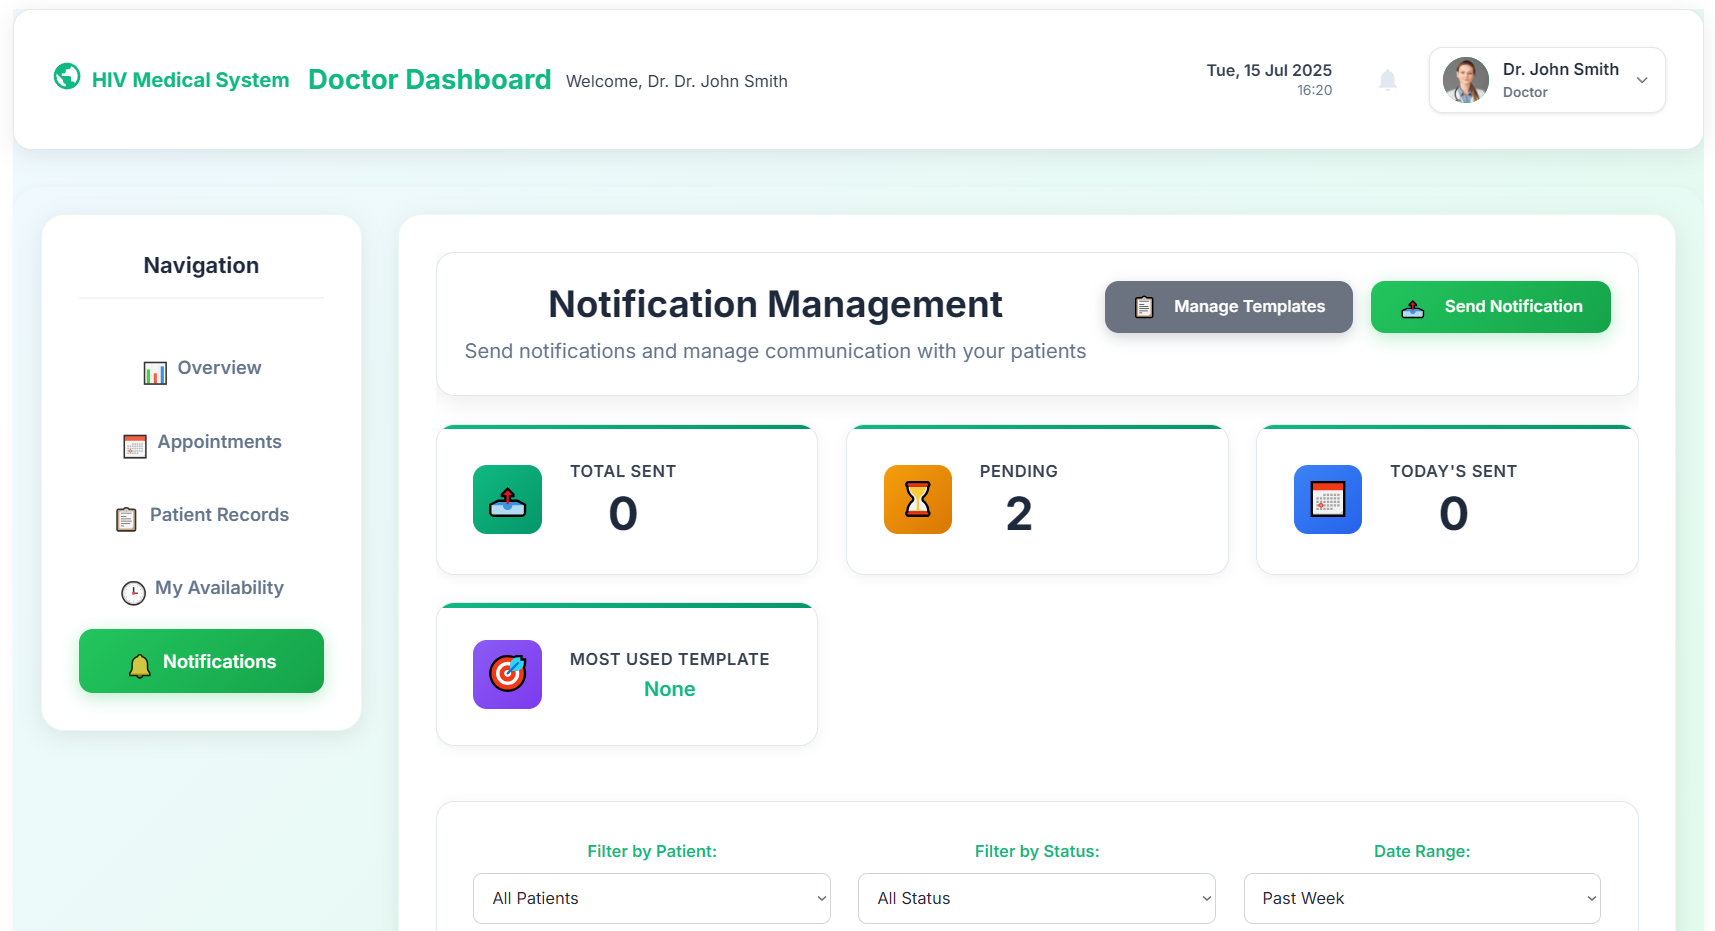
\includegraphics[width=0.9\textwidth]{images/doctor_treatment.png}
\caption{Doctor Treatment Management Interface}
\label{fig:doctor-treatment}
\end{figure}

\subsection{Administrative Functions}

\begin{enumerate}
    \item \textbf{User Management:}
    \begin{itemize}
        \item Login as admin user
        \item Navigate to "User Management"
        \item View all system users
        \item Create new user accounts
        \item Modify user roles and permissions
        \item Deactivate or delete users
        \item Reset user passwords
    \end{itemize}
    
    \item \textbf{System Settings:}
    \begin{itemize}
        \item Access "System Settings" menu
        \item Configure notification templates
        \item Set system-wide preferences
        \item Manage notification schedules
        \item Configure email settings
        \item Update system parameters
    \end{itemize}
\end{enumerate}

\subsection{Notification System}

\subsubsection{Appointment Reminders}

The system automatically sends appointment reminders:
\begin{itemize}
    \item 24 hours before appointment
    \item 1 hour before appointment
    \item 30 minutes before appointment
\end{itemize}

\subsubsection{Medication Reminders}

Patients receive daily medication reminders:
\begin{itemize}
    \item Based on prescribed medication routines
    \item Customizable reminder times
    \item Adherence tracking
    \item Missed dose notifications
\end{itemize}

\subsection{Security Features}

\subsubsection{Data Protection}

\begin{itemize}
    \item JWT token-based authentication
    \item Role-based access control
    \item Password encryption (BCrypt)
    \item Session timeout management
    \item Audit trail for all activities
\end{itemize}

\subsubsection{Privacy Controls}

\begin{itemize}
    \item Patient-controlled data visibility
    \item HIPAA-compliant data handling
    \item Secure data transmission (HTTPS)
    \item Regular security audits
    \item Data backup and recovery
\end{itemize}

\section{Troubleshooting}

\subsection{Common Issues}

\begin{longtable}{@{}|p{4cm}|p{5cm}|p{5cm}|@{}}
\hline
\textbf{Issue} & \textbf{Cause} & \textbf{Solution} \\
\hline
Login failed & Invalid credentials & Check username/password, reset if needed \\
\hline
Database connection error & SQL Server not running & Start SQL Server service \\
\hline
Frontend not loading & Backend not started & Start backend service first \\
\hline
Port already in use & Service conflict & Stop existing service or change port \\
\hline
API requests failing & CORS configuration & Check backend CORS settings \\
\hline
\end{longtable}

\subsection{Support Information}

\begin{itemize}
    \item \textbf{Technical Support:} Check application logs for detailed error messages
    \item \textbf{Documentation:} Refer to README.md for additional setup instructions
    \item \textbf{Database Issues:} Verify SQL Server installation and configuration
    \item \textbf{Network Issues:} Check firewall settings and port availability
\end{itemize}

\section{System Specifications}

\subsection{Technical Requirements}

\begin{longtable}{@{}|p{3cm}|p{4cm}|p{7cm}|@{}}
\hline
\textbf{Component} & \textbf{Specification} & \textbf{Notes} \\
\hline
Operating System & Windows 10+, Linux, macOS & Cross-platform compatibility \\
\hline
Web Browser & Chrome 90+, Firefox 88+, Safari 14+ & Modern browser required \\
\hline
Memory & 8GB RAM minimum & 16GB recommended for development \\
\hline
Storage & 2GB available space & Additional space for database \\
\hline
Network & Internet connection & Required for some features \\
\hline
\end{longtable}

\subsection{Performance Metrics}

\begin{itemize}
    \item \textbf{Response Time:} < 2 seconds for typical operations
    \item \textbf{Concurrent Users:} Supports 100+ concurrent users
    \item \textbf{Database Capacity:} Handles 10,000+ patient records
    \item \textbf{Uptime:} 99.9% availability target
\end{itemize}

\section{Conclusion}

The HIV Clinic Management System v1.0 provides a comprehensive solution for HIV patient care management. The system successfully implements all planned features including appointment booking, patient record management, ARV treatment tracking, and automated notification systems.

Key achievements include:
\begin{itemize}
    \item Secure role-based access control
    \item Comprehensive patient data management
    \item Automated appointment and medication reminders
    \item Intuitive user interfaces for all roles
    \item Robust database design with audit trails
    \item Scalable architecture for future enhancements
\end{itemize}

The system is ready for production deployment and can be extended with additional features as needed.

\end{document}